\textbf{1.  ¿Cree usted que es necesaria una herramienta que ayude a las OE a realizar el proceso de Solicitud de Fondo por Rendir?}

    \begin{figure}[h!]
        \centering
        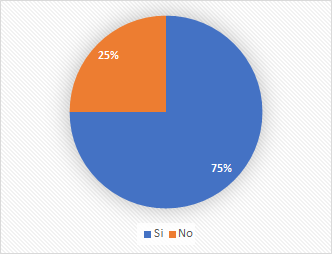
\includegraphics[width=0.6\textwidth]{Imagenes/Pregunta1.png}
        \caption{\label{fig: Pregunta1}Resultado de la pregunta uno.}
    \end{figure}
\newpage
\textbf{2.  ¿Cree usted que esta herramienta puede ayudar a reducir el tiempo que demanda realizar una rendición? (En escala de 1 (No es de ayuda) a 5 (Es de mucha ayuda))}

\begin{figure}[h!]
    \centering
    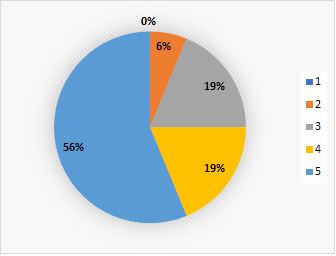
\includegraphics[width=0.55\textwidth]{Imagenes/Pregunta2.png}
    \caption{\label{fig: Pregunta2}Resultado de la pregunta dos.}
\end{figure}

\textbf{3.  ¿Cree usted que la mayoría de las personas pueden aprender a usar el sistema rápidamente? (En escala de 1 (En desacuerdo) a 5 (De acuerdo))}

\begin{figure}[h!]
    \centering
    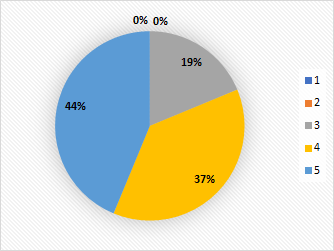
\includegraphics[width=0.55\textwidth]{Imagenes/Pregunta3.png}
    \caption{\label{fig: Pregunta3}Resultado de la pregunta tres.}
\end{figure}

\newpage
\textbf{4.  ¿Cree usted que gracias a la aplicación se puede reducir la causa de rechazo de la Rendición? (En escala de 1 (En desacuerdo) a 5 (De acuerdo))}

\begin{figure}[h!]
    \centering
    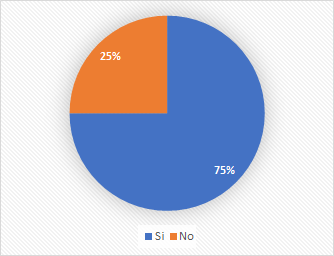
\includegraphics[width=0.55\textwidth]{Imagenes/Pregunta4.png}
    \caption{\label{fig: Pregunta4}Resultado de la pregunta cuatro.}
\end{figure}
